\section{Contextual constraints}\label{sec:contextualconstraints}
The grammar of Arc is a \gls{cfg} and only expresses the structure of the language. Further contextual constraints are required to specify if a program is well-formed and meaningfully correct. This section describes Arc's contextual constraints: the scope- and type rules.

\subsection{Scope rules}\label{subsec:scoperules}
The scope rules govern visibility, hiding some parts of a program from others. It also rules where certain things are allowed and others are not.

The Arduino language has static scope, with nested and flat block structures~\cite{cppref}. Blocks are declarable within other blocks (nested), but functions within other functions are not (flat). Arc will have similar scope rules, making compilation more straightforward as source code and target code resemble each other when it comes to scope. Figure~\ref{fig:arcscoperules} shows a graphical model of Arc's scope rules.


\begin{figure}[htbp]
    \centering
    \begin{tikzpicture}[
            double/.style={draw, anchor=text, rectangle split,rectangle split parts=2},
            triple/.style={draw, anchor=text, rectangle split,rectangle split parts=3}
        ]
        \node[state,align=center] at (14,0) {Global scope \\
            \tikz{\node[double, align=center]{Function declaration scope \\
                    \tikz{\node[state, align=center] {block scopes \\
                            \tikz{\node[state, align=center] {block scope}}
                        }
                    }
                    \nodepart{second}Task declaration scope \\
                    \tikz{\node[state, align=center] {block scopes}
                    }}}
        };
    \end{tikzpicture}
    \caption{Diagram of the scope structure of Arc.}
    \label{fig:arcscoperules}
\end{figure}


Arc statements and blocks, therefore, have nested scoping, while function declarations have flat scope and are not declarable inside a scope. However, one key feature of Arc is its \textit{task} construct, which is not present in Arduino and requires particular focus.

A task declaration is like a function declaration and cannot be inside another scope. Additionally, declaring local variables inside the scope of a task declaration is not possible. The Protothreads implementation does not guarantee that the values of local variables are preserved when a thread becomes blocked, making it hard to know if using local variables in a thread will work as the programmer intended.

Another solution to this problem could be to hoist local variable declarations within a task declaration into the global scope. However, this could make static scopechecking more difficult. Listing~\ref{lst:hoistclash} shows how the hoisting of a locally declared variable may clash with globally declared variables. While the hoisting issue is not unsolvable, it is clearer to disallow variable declarations within a task declaration. Most importantly, writing an Arc task is entirely declarative - tasks are never called, unlike functions.


\begin{listing}[htb!]
    \begin{minted}[label=Scope clash]{text}
        num a = 1;
        task() {
            num a = 2; // hoist causes a clash here
        }
    \end{minted}
    \caption{Example of hoisting that causes a clash.}
    \label{lst:hoistclash}
\end{listing}


To describe the static scope rules of Arc with operational semantics, we use the environment-store model from Figure~\ref{fig:envstomodel}. The environment-store model describes variables as binding to locations, and locations binding to values, while the locations and values are then read with partial functions called \textit{environment} and \textit{store}.


\begin{figure}[htb!]
    \centering
    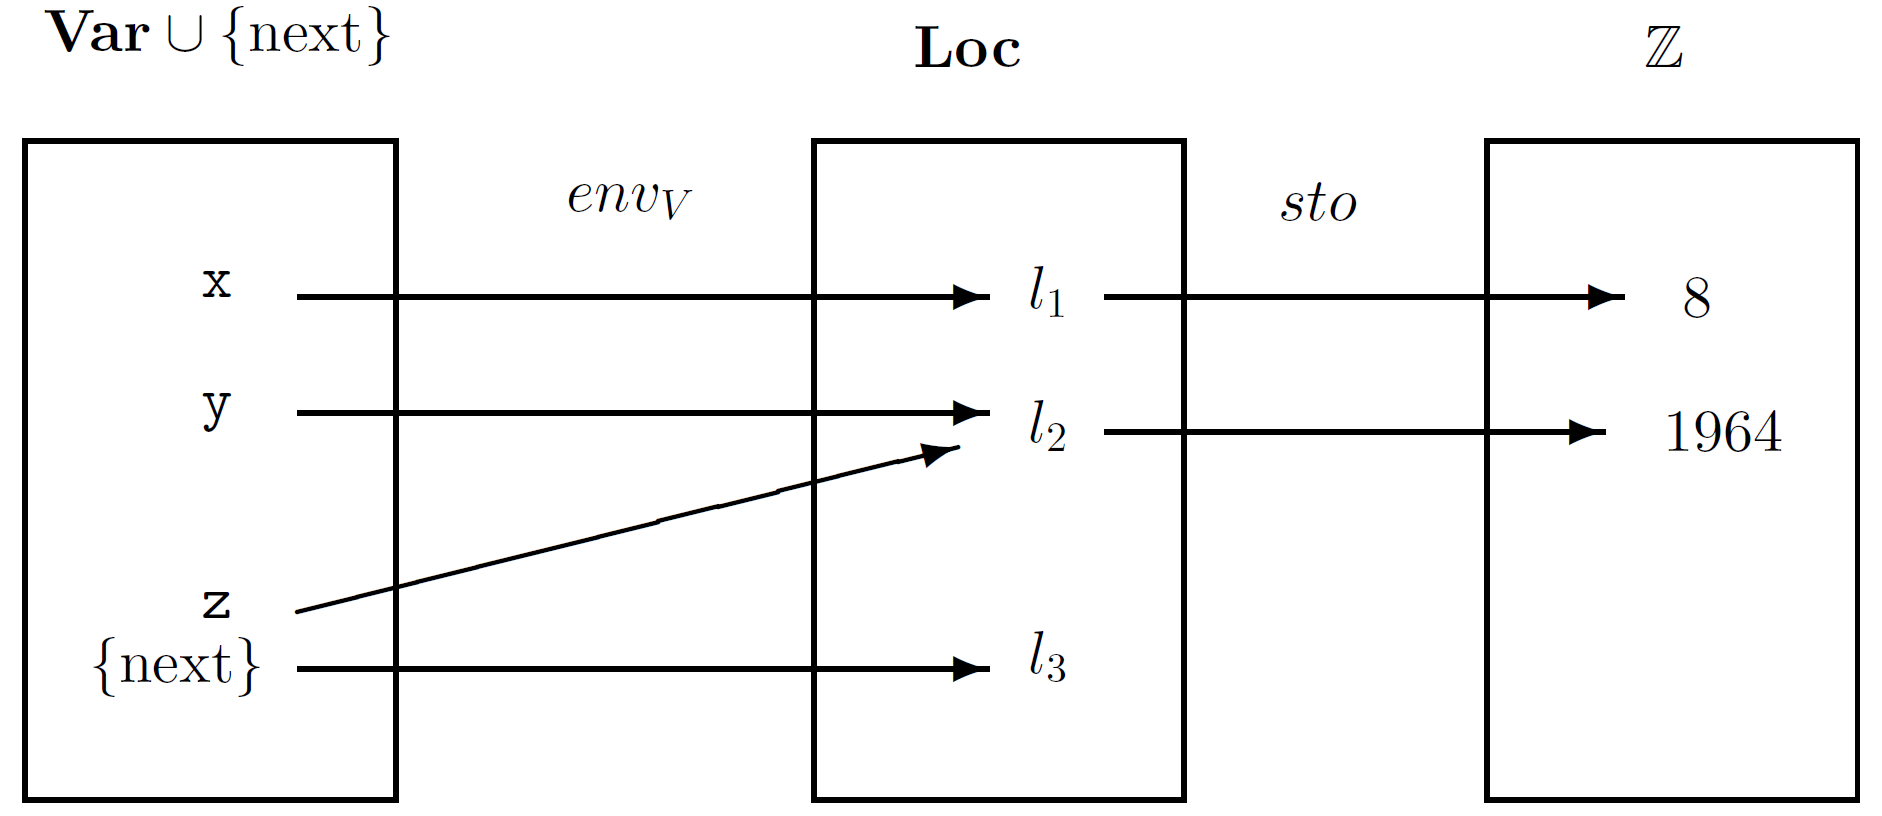
\includegraphics[width=0.8\textwidth]{figures/Environment_Store.png}
    \caption{Example diagram of the environment store model~\cite{Huttel2010}.}
    \label{fig:envstomodel}
\end{figure}


Arc has three environments: the variable environment, the function environment, and the task environment. To describe the semantics of these environments, some function, set and value names must be defined first. These definitions are presented in Table~\ref{tab:setsandfunctions}, and correspond to rules of Arc's \gls{cfg} described mathematically.

Following the standard of~\cite{Huttel2010}, sets are bolded and begins with a capital letter, while elements are not bolded.


\begin{table}[htb!]
    \centering
    \begin{tabular}{l}
        \toprule
        $\textbf{Val} = \textbf{Num} \cup \textbf{Bool} \cup \textbf{Char} \cup \textbf{Array} \cup \textbf{Pin}\ -$ Values                                                        \\
        $\textbf{Pin} = \textbf{PinValues} \times \textbf{Modes}\ -$ Pins are tuples of Arduino pins and modality                                                                  \\
        $\textbf{Array} = \mathbb{N} \rightharpoonup \textbf{Val} \setminus \textbf{Pin}\ -$ Arrays map numbers to non-pin values                                                  \\
        $\textbf{Par} = \textbf{Types} \times \textbf{Var}\ -$ Set of possible formal parameters                                                                                   \\
        $\textbf{Trig} = \{\epsilon, (\text{every} \times \mathbb{N}), (\text{when} \times \textbf{Expr}) \}\ -$ Set of triggers                                                   \\
        $v \in \textbf{Val}\ -$ Literal values                                                                                                                                     \\
        $x \in \textbf{Var}\ -$ Variable id                                                                                                                                        \\
        $f \in \textbf{Fun}\ -$ Function id                                                                                                                                        \\
        $t \in \textbf{Types}\ -$ Type names                                                                                                                                       \\
        $y \in \mathcal{P} (\textbf{Par})\ -$ Formal parameter lists                                                                                                               \\
        $r \in \mathcal{P} (\textbf{Var})\ -$ Reference parameter lists                                                                                                            \\
        $S \in \textbf{Stm}\ -$ Statements                                                                                                                                         \\
        $l \in \textbf{Loc}\ -$ An arbitrary location in \textbf{Loc}                                                                                                              \\
        next $\ -$ A special 'pointer' holding the value of the next element in \textbf{Loc}                                                                                       \\
        new $: \textbf{Loc} \rightarrow \textbf{Loc}\ -$ function to return succesor location                                                                                      \\
        \\
        $\textbf{Sto} = \textbf{Loc} \rightharpoonup \textbf{Val}\ -$ Set of stores                                                                                                \\
        $\textbf{Env}_V = \textbf{Var} \cup \{\text{next}\} \rightharpoonup \textbf{Loc}\ -$ Set of variable environments                                                          \\
        $\textbf{Env}_F = \textbf{Fun} \rightharpoonup \textbf{Stm} \times \mathcal{P} (\textbf{Par}) \times \textbf{Env}_V \times \textbf{Env}_F\ -$ Set of function environments \\
        $\textbf{Env}_T = \textbf{Stm} \times \mathcal{P} (\textbf{Var}) \times \textbf{Trig} \times \textbf{Env}_V \times \textbf{Env}_F\ -$ Set of task environments             \\
        \bottomrule
    \end{tabular}
    \caption{Sets and function definitions.}
    \label{tab:setsandfunctions}
\end{table}

\supervisor{Should we define types as $\{\epsilon, mut\} \times \textbf{Typenames} \cup \textbf{Typenames}$}


Additionally, we define the notation for updating a given environment $env_V \in \textbf{Env}_V$ we write $env_V[ x \mapsto l]$ to denote the update of $env_V$ given by


\begin{equation}
    env_V[x \mapsto l](y) =
    \begin{cases}
        env_V(y) & y \neq x \\
        l        & y = x
    \end{cases}
\end{equation}


\noindent and $env_F[ f \mapsto (S, y, env_V, env_F)]$ for $env_F$


\begin{equation}
    env_F[f \mapsto (S, y, env_V, env_F)](g) =
    \begin{cases}
        env_F(g)             & g \neq f \\
        (S, y, env_V, env_F) & g = f
    \end{cases}
\end{equation}


\noindent and similarly for a $sto \in \textbf{Sto}$ we write $sto[ l \mapsto v ]$ to indicate the update of $sto$ given by


\begin{equation}
    sto[l \mapsto v](l^\prime) =
    \begin{cases}
        sto(l) & l \neq l^\prime \\
        v      & l = l^\prime
    \end{cases}
\end{equation}
\todo{Missing $env_T$ definition. Should just be a set union an element.}

\noindent With the above definitions of the environment store model and the scope rules, Arc's declarations are described using operational semantics in Table~\ref{tab:arcscoperules}. Because of the static scope rules, the environments are contained within the results of the partial functions for variables and functions. Unlike the variable and function environments, the task environment is not a set of partial functions. This is because unlike function declarations, tasks are not used within other tasks, and as such does not need to map them.


\begin{table}[htb!]
    \small
    \centering
    \begin{tabular}{ll}
        \toprule
        $[PIN_{DECL}]$  & $\frac
            {\langle env^{\prime\prime}_V, sto[l \mapsto v] \rangle \rightarrow (env^\prime_V, sto^\prime)}
            {\langle \text{\#pin} \ x = (pv, mode), env_V, sto\rangle\rightarrow (env^\prime_V, sto^\prime)}$ \\ [12pt]
                        & where $(pv, mode) \in \textbf{Pin} $                                                \\
                        & and $(pv,mode) \rightarrow v $                                                      \\
                        & and $l = env_V(\text{next})$                                                        \\
                        & and $env^{\prime\prime}_V = env_V[x \mapsto l][\text{next} \mapsto \text{new}(l)] $ \\
        \\

        $[VAR_{DECL}]$  & $\frac
            {\langle env^{\prime\prime}_V, sto[l \mapsto v] \rangle \rightarrow (env^\prime_V, sto^\prime)}
            {\langle t \ x = expr, env_V, sto\rangle\rightarrow (env^\prime_V, sto^\prime)}$                  \\ [12pt]
                        & where $env_V, sto \vdash expr \rightarrow v $                                       \\
                        & and $l = env_V(\text{next})$                                                        \\
                        & and $env^{\prime\prime}_V = env_V[x \mapsto l][\text{next} \mapsto \text{new}(l)] $ \\
        \\

        $[FUNC_{DECL}]$ & $\frac
            {env_V \vdash \langle env_F[f \mapsto \langle S, y, env_V, env_F\rangle] \rangle \rightarrow env^\prime_F}
            {env_V \vdash \langle t \ f (y) \{S \}, env_F \rangle \rightarrow env^\prime_F}$                  \\ [12pt]

        $[TASK_{DECL}]$ & $\frac
            {env_{VF}\vdash \langle env_T[S, r, trig, env_V, envF] \rangle \rightarrow env^\prime_T}
            {env_{VF}\vdash \langle \text{task} \ (r) trig \{S\} \rangle \rightarrow env^\prime_T}$           \\
        \bottomrule
    \end{tabular}
    \caption{Arc's declarations and effects on scope defined with operational semantics.}
    \label{tab:arcscoperules}
\end{table}


To use the declared bindings we further define their calling and usage. Variables are immutable, and it therefore makes sense to have functions use call-by-value for the parameters. Function calls should not allow recursion, as this makes the runtime memory usage of the Arduino more stable.

Tasks are once again special. They are never called explicitly in Arc code, but the set of all declared tasks serve as the entrypoint of the program. This is done through parallel composition and invocation of all declared tasks, of which there must be at least one.

Also of importance is that the parameters of a task describe a mutable reference to a declared variable in $env_V$, that critically cannot be used in another task. This means that declarations are implicit calls with a call-by-reference model for its parameters.


\begin{table}[htb!]
    \centering
    \begin{tabular}{ll}
        \toprule
        $FUNC_{CALL}$ & $\frac{}{env_{VF} \vdash \langle f(e), sto\rangle \rightarrow sto^\prime}$ \\ [12pt]
                      & where $env_F(f) = \langle S, y, env^\prime_V, env^\prime_F \rangle$        \\
                      & and $\forall i | 0 \leq i \leq |y|$                                        \\
                      & and $e \in \textbf{Expr}^{ |y| }$                                          \\
                      & and $\forall i $                                                           \\

        $ENTRY$       & $\frac{}{}$                                                                \\ [12pt]
        \bottomrule
    \end{tabular}
    \caption{Semantics for function calls and task invocation.}
    \label{tab:callandentry}
\end{table}
\supervisor{How do I describe that each expression in the parameter list is evaluated and stored in a new location, with a variable $y_i$ from the formal parameter list pointing to that location?!}


\subsection{Type rules}\label{subsec:typerules}
Type rules are another set of contextual constraints. These rules make sure that code fragments do not mistreat types, for example in static typing, which Arc uses, it should not be possible to assign a number to a variable declared as a boolean~\cite{Sebesta2016}. The types that are valid in Arc are num, char, bool, and array, as descriped in~\ref{sec:inspiration}.

In the type checking semantics the types in the Arc language can be written as:
$T \in \{num, char, bool, N\} N \in \{ 0,\mathbb{N}\}$.
From now on semantics written mathmatticly will use T instead of type, if not given a specific type, in semantic type checking. If a specific type is needed, it is written instead of T.
N is not descriped ealier on what the types are in Arc, as it is not a type that can be declared. N is used for accessing an array, In C++ array access has to have a natural number, this is also implemented in Arc aswell. In C++ it is also 0-indexed~\cite{cppreferenceDataTypes}, which is withhold in Arc aswell.
In declarations and statements type checking, there will be an evaluation to $ok$ which means:

\blockcquote{Huttel2010}{The type of a declaration or a statement will simply be ok; we say that the declaration or statement is well-typed}

In Table~\ref*{tab:DeclTypeCheck}, the type checking for variables and functions are written. A specific type function declaration, has to type check if the return type is the same type as the declared function type. As task and a void function do not return, these declarations are always well-typed.


\begin{table}[htb!]
    \centering
    \begin{tabular}{ll}
        \toprule
        $[VAR_{DECL}] $  & $\frac{env \vdash expr : T}{env \vdash T \;x = expr : ok}$                            \\  [12pt]
        $[FUNC_{DECL}] $ & $\frac{env \vdash expr : T}{env \vdash T \;f() \{S; \;\text{return} \; expr\}  : ok}$ \\  [12pt]
        $[VOID_{DECL}] $ & $f()\{S\}  : ok$                                                                      \\
        \bottomrule
    \end{tabular}
    \caption{Arc type check for declarations.}
    \label{tab:DeclTypeCheck}
\end{table}


Now that the types has been clarified, it is important to look at operations a specific type can do.
The first type that will be clarified is num.
In Table~\ref{tab:num-rules} the expressions which the data type num only can do, is showed here.


\begin{table}[htb!]
    \centering
    \begin{tabular}{lll}
        \toprule
        $[ADD_{EXPR}] $                         & $\frac
            {env\vdash expr_1: num \quad env\vdash expr_2: num}
            {env\vdash expr_1 \;+\;expr_2: num}$
        \\ [12pt]
        $[SUB_{EXPR}] $                         & $\frac
            {env\vdash expr_1: num \quad env\vdash expr_2: num}
            {env\vdash expr_1 \;-\;expr_2: num}$
        \\ [12pt]
        $[MULT_{EXPR}] $                        & $\frac
            {env\vdash expr_1: num \quad env\vdash expr_2: num}
            {env\vdash expr_1 \;*\;expr_2: num}$
        \\ [12pt]
        $[DIVI_{EXPR}] $                        & $\frac
            {env\vdash expr_1: num \quad env\vdash expr_2: num}
        {env\vdash expr_1 \; / \; expr_2: num}$ & where $expr_2 \neq 0$
        \\ [12pt]
        $[REL_{EXPR}] $                         & $\frac
            {env\vdash expr_1: num \quad env\vdash expr_2: num}
            {env\vdash expr_1 \; OP \; expr_2: Bool}$                                 \\

                                                & where $OP \in \{<, >, \leq, \geq\}$

        \\
        \bottomrule
    \end{tabular}
    \caption{Type rules for num expressions in Arc.}
    \label{tab:num-rules}
\end{table}


The type num is the only type in Arc that can do arithmetic expressions, as it can only do arithmetic expressions on another num type, this can be seen in Table~\ref{tab:num-rules}. The end type of a arithmetic expression is still a num, as it makes changes to the value, not the type.

It is also the only type to check if a value is greater or smaller than an other num type when comparing. When doing a comparing of nums, the end type of the expression is a bool, as it true or false if the num is greater or less than the num it is compared to.


\begin{table}[htb!]
    \centering
    \begin{tabular}{ll}
        \toprule
        $[AND_{EXPR}] $ & $\frac
            {env\vdash expr_1: Bool \quad env\vdash expr_2: Bool}
            {env\vdash expr_1 \;\text{and} \;expr_2: Bool}$
        \\ [12pt]
        $[OR_{EXPR}] $  & $\frac
            {env\vdash expr_1: Bool \quad env\vdash expr_2: Bool}
            {env\vdash expr_1 \;\text{or} \;expr_2: Bool}$
        \\ [12pt]
        $[NOT_{EXPR}] $ & $\frac
            {env\vdash expr_1: Bool}
            {env\vdash \text{not} \; expr_1 : Bool}$
        \\
        \bottomrule
    \end{tabular}
    \caption{Type rules for bool expressions in Arc.}
    \label{tab:bool-rules}
\end{table}


The type bool has three expressions, that can be seen in Table~\ref{tab:bool-rules}. This means in the And, Or or Not expressions the expression getting type checked has to evaluate to a bool, the expressions will then evaluate to another type bool.


\begin{table}[htb!]
    \centering
    \begin{tabular}{ll}
        \toprule
        $[ARRAY_{EXPR}]$      & $ \frac
            {env\vdash expr_1: T \quad env \vdash expr_2 : N}
            {env\vdash expr_1[expr_2] : T}$
        \\ [12pt]
        $[PARENTHESIS{EXPR}]$ & $ \frac
            {env\vdash expr_1: T}
            {env\vdash (expr_1) : T}$
        \\ [12pt]
        $[EQUAL_{EXPR}] $     & $\frac
            {env\vdash expr_1: T \quad env\vdash expr_2: T}
            {env\vdash expr_1 \;== \;expr_2: Bool}$
        \\ [12pt]
        $[NOTEQUAL_{EXPR}] $  & $\frac
            {env\vdash expr_1: T \quad env\vdash expr_2: T}
            {env\vdash expr_1 \;!= \;expr_2: Bool}$
        \\
        \bottomrule
    \end{tabular}
    \caption{Type rules for other types of expressions in Arc.}
    \label{tab:expr-rules}
\end{table}


The type char does not have any expressions that only can be used on that type, therfore it only can use the expressions which bool and num can do as well. These type rules for expressions is written on Table~\ref{tab:expr-rules}. In the array expression the type N is used to describe the index for the array. The equal and not equal expression evaluate to a bool type, as it can only be true or false.


\begin{table}[htb!]
    \centering
    \begin{tabular}{ll}
        \toprule
        $[COMP_{STMT}] $     & $\frac
            {env \vdash stmt_1 :ok \quad env \vdash stmt_2 :ok}
            {env \vdash stmt_1\;;\;stmt_2: ok}$
        \\ [12pt]
        $[VAR-DECL_{STMT}] $ & $\frac
            {env \vdash expr : T}
            {env \vdash  T \;x = expr: ok}$
        \\ [12pt]
        $[ASSIGN_{STMT}]$    & $\frac
            {env\vdash x: T \quad env \vdash expr : T}
            {env\vdash x = expr: ok}$
        \\ [12pt]
        $[INDEX_{STMT}] $    & $\frac
            {env \vdash x : T \quad env \vdash expr : N \quad env \vdash expr : T}
            {env \vdash x[expr] = expr: ok}$
        \\ [12pt]
        $[BLOCK_{STMT}] $    & $\frac
            {env \vdash stmt :ok}
            {env \vdash \{stmt\}: ok}$
        \\ [12pt]
        $[CALL_{STMT}] $     & $\frac
            {env \vdash f:(x:T \rightarrow ok)\quad env \vdash expr:ok}
            {env \vdash call \;f(expr): ok}$
        \\ [12pt]
        $[RETURN_{STMT}] $   & $\frac
            {env \vdash expr: T}
            {env \vdash \text{return} \;expr: ok}$
        \\ [12pt]
        $[IF_{STMT}] $       & $\frac
            {env \vdash if (expr) : Bool \quad env \vdash stmt_1 :ok \quad env \vdash stmt_2 :ok}
            {env \vdash \text{if} (expr) \;stmt_1 \;\text{else} \;stmt_2: ok}$
        \\ [12pt]
        $[WHILE_{STMT}] $    & $\frac
            {env \vdash  expr : Bool \quad env \vdash stmt :ok}
            {env \vdash \text{while} (expr) \;stmt : ok}$
        \\ [12pt]
        $[FOR_{STMT}] $      & $\frac
            {env \vdash  y : T \quad env \vdash x : T \quad env \vdash block :ok}
            {env \vdash \text{for} (y \; \text{in} \; x) \; block : ok}$
        \\
        \bottomrule
    \end{tabular}
    \caption{Arc type check statements.}
    \label{tab:StatementTypeCheck}
\end{table}


The type checking for statements in Arc can be seen in Table~\ref{tab:StatementTypeCheck}. Type checking statements gives the same output as the declarations in "ok", as explained before means well-typed. A varable can be declared in a scope, therfore it has the same type check rules as in variable declaration, which can be seen in Table~\ref{tab:DeclTypeCheck}. Return uses an expression which evaluates to a type "T", this type is the same type as the type a function is declared with.
